\section{图的基本概念}
\label{sec:graph-basic-concepts}

一张道路网只需回答“哪些城市之间有一条直达道路”，一份任务清单只需回答“哪项任务直接依赖哪项任务”。两者的共同之处是：对象有限，信息集中在成对对象之间的直接连接上。本节先把这种信息写成图，再分别说明方向、数值和属性给连接添加了什么，最后讨论从一张图中取出一部分时保留了什么。

\subsection{图的定义}
\label{sec:graph-conn-definition}

把每个对象记为一个顶点，把每一对有直接连接的对象记为一条边，就得到一张图。这里先考虑没有方向的连接，例如可以双向通行的道路。

\begin{definition}[图]
\label{def:graph-conn-graph}
设$V$是有限集合，$E$是由$V$中两个不同元素组成的无序对$\{i,j\}$的集合，称$\mathcal G=(V,E)$为一个（无向）\term{图}（graph）。$V$中的元素称为\term{顶点}（vertex），$E$中的元素称为\term{边}（edge）。若$\{i,j\}\in E$，称$i,j$是这条边的两个端点。
\end{definition}

记$n=|V|$为顶点数，$m=|E|$为边数。全章使用同一个例子：
\begin{equation}
V=\{1,2,3,4\},\qquad
E=\bigl\{\{1,2\},\{1,3\},\{2,3\},\{2,4\},\{3,4\}\bigr\},
\label{eq:graph-conn-running-graph}
\end{equation}
它有$n=4$个顶点、$m=5$条边，可以看成两个三角形$\{1,2,3\}$与$\{2,3,4\}$共用边$\{2,3\}$。四个顶点之间最多有$\binom42=6$条边，这里只缺$\{1,4\}$。

\paragraph{图与画法}
图只由集合$V$和$E$确定，纸上的画法不属于图。图~\ref{fig:graph-conn-running-drawings}把同一张图画了三次：顶点的位置不同，线段的长短和弯曲不同，(c)中两条边还在画面上交叉，但三幅图的顶点集和边集完全相同，因此是同一张图。交叉点不是顶点，线段长度也不是边的长度；如果问题需要长度、坐标或其他数值，必须另外指定，见第~\ref{sec:graph-conn-weights}小节。

\begin{figure}[!htb]
  \centering
  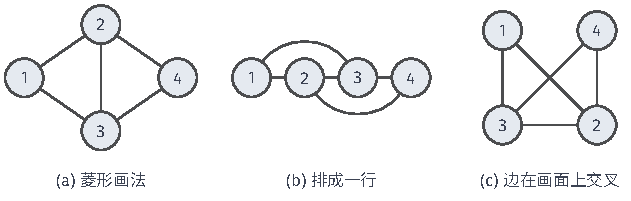
\includegraphics[width=106.765mm]{figures/01-basic-mathematics/04-graphs/tikz/c1-running-graph-drawings/figure.pdf}
  \caption{贯穿全章的四点五边图\eqref{eq:graph-conn-running-graph}的三种画法。顶点位置、线段形状和交叉情况都不同，但边集都是$\{1,2\},\{1,3\},\{2,3\},\{2,4\},\{3,4\}$。(c)中两条对角边在画面上交叉，交叉处不是顶点。}
  \label{fig:graph-conn-running-drawings}
\end{figure}

\paragraph{简单图的约定}
定义~\ref{def:graph-conn-graph}要求边的两个端点不同，并且边集是普通集合，因此排除了两种情形：一个顶点连到自身的\term{自环}（self-loop），以及同一对顶点之间的多条\term{平行边}（parallel edges）。满足这两条限制的图称为\term{简单图}（simple graph），本部分默认讨论有限简单图。若实际问题需要两条平行道路分别记录收费，就要给每条边一个独立身份，不能再把边等同于端点对；这时后面诸如“$n$个顶点最多有$\binom n2$条边”的计数也不再成立。用到这类扩展时会明确指出。

顶点集为空的图只有空边集，它在少数边界情形中出现，例如删除全部顶点后的余图。凡是结论需要至少一个顶点，我们都会写明“非空图”。

\subsection{无向图与有向图}
\label{sec:graph-conn-directions}

道路可以双向通行，“任务$i$完成后才能开始任务$j$”却有先后。无序对$\{i,j\}$不区分两个端点的次序，不能记录后一种信息，因此需要有序对。

\begin{definition}[有向图]
\label{def:graph-conn-digraph}
设$V$是有限集合，$E\subseteq\{(i,j)\in V\times V:i\neq j\}$，称$\mathcal G=(V,E)$为\term{有向图}（directed graph）。有序对$(i,j)\in E$称为从$i$到$j$的\term{弧}（arc），也记作$i\to j$；$i$是它的起点，$j$是它的终点。
\end{definition}

为了区分，以无序对为边的图也称\term{无向图}（undirected graph）。有向图的弧集仍记作$E$，弧数仍记作$m$；需要强调时再说“边或弧”。弧$i\to j$只允许从$i$一步到达$j$，并不包含反向的$j\to i$。

\paragraph{一条无向边不等于两条反向弧}
图~\ref{fig:graph-conn-direction-orientation}(a)(b)对照了无向边$\{u,v\}$与一对反向弧$(u,v),(v,u)$。两者都允许在$u,v$之间来回，但建模含义不同：无向边是一条连接，删除它就同时失去两个方向；两条弧则是两个独立对象，可以只删除其中一条，也可以分别附上不同的数值，例如上坡与下坡的不同用时。把无向图改写成有向图时，可以用一对反向弧代替每条边，但要记住这一步改变了“边”的个数和身份。

\paragraph{方向改变可达的范围}
图~\ref{fig:graph-conn-direction-orientation}(c)--(e)给同一条三点连接1—2—3赋予不同方向。无向时三个顶点两两可以互相到达；定向为$1\to2\to3$后，从$1$可以经$2$到达$3$，从$3$却哪里也去不了；定向为$1\to2\leftarrow3$后，$1$和$3$都只能到达$2$，彼此不能到达。可见方向不只是标注，它直接决定哪些顶点序列允许通行。

\begin{figure}[!htb]
  \centering
  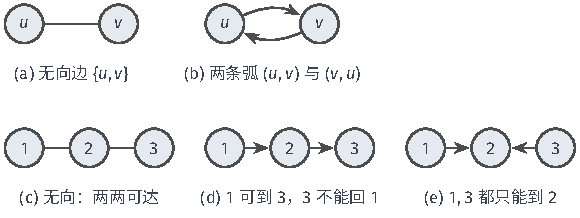
\includegraphics[width=98.189mm]{figures/01-basic-mathematics/04-graphs/tikz/c1-direction-orientation/figure.pdf}
  \caption{方向给连接附加的信息。上排：一条无向边与一对反向弧都允许在$u,v$之间往返，但后者的两条弧可以分别删除或另附数值。下排：同一条三点连接的无向形式(c)与两种定向(d)(e)，箭头决定了从哪个顶点能走到哪个顶点。}
  \label{fig:graph-conn-direction-orientation}
\end{figure}

\paragraph{底层无向图}
忽略有向图每条弧的方向，把$(i,j)$与$(j,i)$都换成无序对$\{i,j\}$（两者同时出现时只留一条边），得到的无向图称为原图的\term{底层无向图}（underlying undirected graph）。图~\ref{fig:graph-conn-direction-orientation}中(d)(e)的底层无向图都是(c)。这一步丢掉了依赖的先后：(c)中$3$能到达$1$，(d)中却不能，所以不能根据底层无向图的连接情况断言原有向图可以双向到达。第~\ref{sec:graph-connectivity-separation}节的弱连通正是建立在底层无向图上的概念，那里会再次比较两者。

\subsection{边权与属性}
\label{sec:graph-conn-weights}

图只说明哪些顶点直接相连。许多问题还需要每条连接上的一个数：道路有多长，管道每秒最多输送多少，两个样本有多相似。

\paragraph{边权的三种常见语义}
给每条边$\{i,j\}$（或弧$(i,j)$）附加一个实数，称为\term{边权}（edge weight）。图~\ref{fig:graph-conn-weight-semantics}在同一个边集上附加了同一组数，却给出三种读法。读作长度$\ell_{i,j}$时，数值沿路线逐条相加，路线$1,2,4$的总长是$2+1=3$，越小越好；读作容量$c_{i,j}$时，数值是通过这条边的流量上限，边$\{1,3\}$上至多通过$1$个单位，容量不沿路线相加；读作相似度$w_{i,j}$时，权重越大，后续计算越强地要求两端取值接近。同一个数字$1$在三种问题里参与的运算完全不同，所以拿到一张带权图时，要先问清权重的用途，再选择方法。

\begin{figure}[!htb]
  \centering
  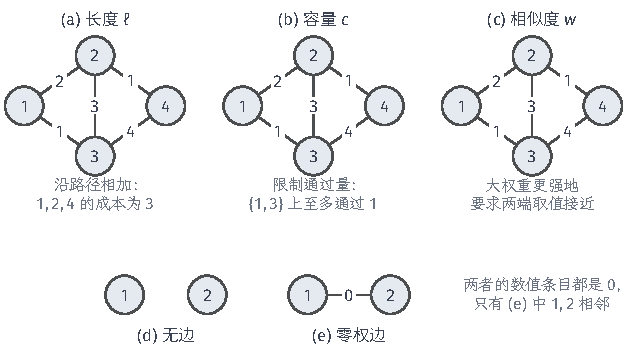
\includegraphics[width=106.768mm]{figures/01-basic-mathematics/04-graphs/tikz/c1-weight-semantics/figure.pdf}
  \caption{同一边集上的同一组边权在三种问题中的读法。(a)长度沿路线相加，路线$1,2,4$的总长为$3$；(b)容量限制单条边的通过量；(c)相似度越大，越要求两端取值接近。下排对照无边(d)与零权边(e)：二者在数值上都记为$0$，但只有(e)中顶点$1,2$相邻。}
  \label{fig:graph-conn-weight-semantics}
\end{figure}

\paragraph{无边与零权边}
边权为$0$并不等于没有边。零长度的道路表示免费通行，零容量的管道不能输送正流量，零相似度在加权求和中不贡献数值；但在这三种情形中，结构上的边都还在。图~\ref{fig:graph-conn-weight-semantics}(d)(e)中，两个顶点之间有没有边由边集决定，与边权是否为零无关：“能否一步到达”查边集，“沿边累计多少”查边权。第~\ref{sec:graph-representations}节用矩阵记录图时，这一区别会变成一个具体的存储问题。

边权能否为负，也由问题决定。负长度可以表示途经某处得到补贴，它会让最短路问题出现新的困难；谱方法则要求相似度非负。这些条件分别在第~\ref{chap:graph-optimization}章和第~\ref{chap:graph-spectral}章建立，本章不预设边权的符号。

\paragraph{顶点属性与边属性}
除了一个实数，边上还可以记录类别、时间等其他数据，顶点上也可以记录人口、坐标等数据，分别称为边属性和顶点属性。顶点的名称$1,2,3,4$只用来区分顶点，本身不是属性：第~\ref{sec:graph-isomorphism}节比较两张图时会看到，换一套名称不改变图的结构，而属性是否必须保持则要由问题声明。

\subsection{子图与诱导子图}
\label{sec:graph-conn-subgraphs}

研究道路网时，常常只关心其中一部分城市，或者想知道封闭几条道路后还剩什么。这两种操作都从原图取出一部分，但保留的东西不同。

\paragraph{子图}
若$V'\subseteq V$，$E'\subseteq E$，并且$E'$中每条边的两个端点都在$V'$中，称$\mathcal G'=(V',E')$是$\mathcal G$的\term{子图}（subgraph）。最后一条要求保证$\mathcal G'$本身仍是一张图，不会出现端点被删掉的边。两种基本操作都产生子图：删除一条边$e$只去掉这条边，顶点全部保留，记作$\mathcal G-e$；删除一个顶点集$S$则去掉$S$中的顶点以及所有至少有一个端点在$S$中的边，记作$\mathcal G-S$。

在图~\ref{fig:graph-conn-subgraph-induced}中，(b)(c)两个子图保留同一组顶点$\{1,2,3\}$，边集却不同：(b)保留三条边，(c)只保留$\{1,2\}$与$\{2,3\}$。所以只给出顶点集合，还不能确定一个一般子图；(d)则是只删除边$\{2,3\}$、保留全部顶点的子图。

\begin{figure}[!htb]
  \centering
  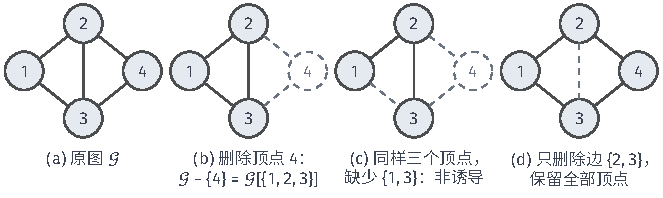
\includegraphics[width=112.000mm]{figures/01-basic-mathematics/04-graphs/tikz/c1-subgraph-induced/figure.pdf}
  \caption{贯穿图的几种子图，灰色虚线表示被删除的顶点或边。(b)删除顶点$4$及其两条边，恰好得到顶点集$\{1,2,3\}$上的诱导子图；(c)保留同样三个顶点，却漏掉了原图中的边$\{1,3\}$，是子图但不是诱导子图；(d)只删除一条边，顶点全部保留。}
  \label{fig:graph-conn-subgraph-induced}
\end{figure}

\paragraph{诱导子图}
只研究一部分顶点时，通常不希望悄悄改变这些顶点之间的关系。为此固定顶点子集，把原图中两端都在其中的边全部保留下来。

\begin{definition}[诱导子图]
\label{def:graph-conn-induced-subgraph}
设$S\subseteq V$。以$S$为顶点集、以$\{\{i,j\}\in E:i,j\in S\}$为边集的子图，称为$\mathcal G$在$S$上的\term{诱导子图}（induced subgraph），记作$\mathcal G[S]$。有向图的诱导子图保留两端都在$S$中的全部弧。
\end{definition}

诱导子图由顶点集唯一确定。图~\ref{fig:graph-conn-subgraph-induced}(b)是$\mathcal G[\{1,2,3\}]$，它必须保留三角形的三条边；(c)虽然顶点相同，但缺少$\{1,3\}$，不是诱导子图。删除顶点与取诱导子图互为补充：$\mathcal G-S=\mathcal G[V\setminus S]$。后面讨论删除一组顶点能否切断连接（第~\ref{sec:graph-connectivity-separation}节），以及第~\ref{chap:graph-traversal}章把图按分隔集分块时，用到的都是这一记号。
